\documentclass{article}
% translate with >> pdflatex -shell-escape <file>

% This file is used as unit test for pgfplots, copyright by Christian Feuersaenger.
% 
% See
%   http://pgfplots.sourceforge.net/pgfplots.pdf
% for pgfplots.
%
% Any required input files (for <plot table> or <plot file> or the table package) can be downloaded
% at
% http://www.ctan.org/tex-archive/graphics/pgf/contrib/pgfplots/doc/latex/
% and
% http://www.ctan.org/tex-archive/graphics/pgf/contrib/pgfplots/doc/latex/plotdata/

\usepackage{pgfplots}
\usepgfplotslibrary{groupplots}
\pgfplotsset{compat=newest}

\pagestyle{empty}

\begin{document}
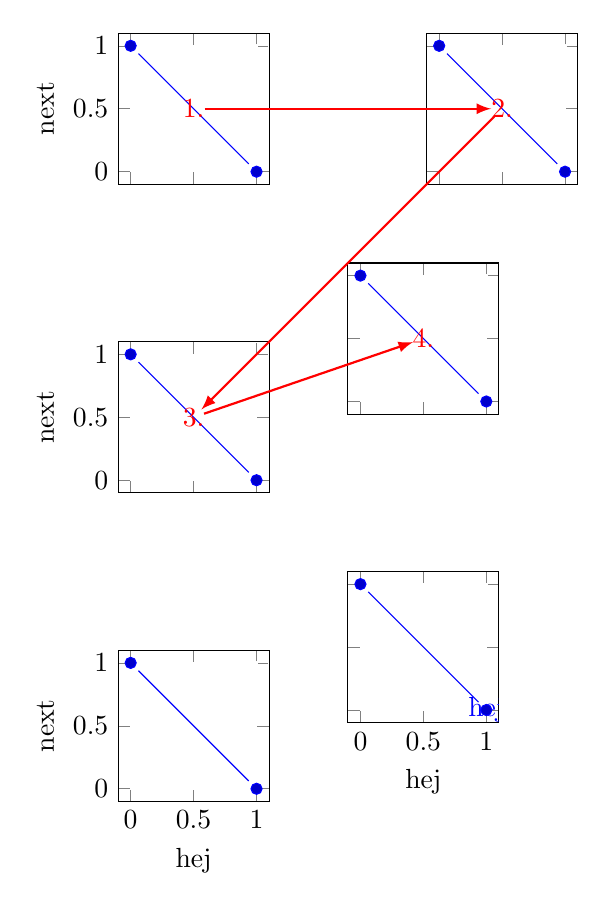
\begin{tikzpicture}[shorten >=4pt,shorten <=4pt]
  \begin{groupplot}[group style={group size=2 by 3,vertical sep=2cm,y descriptions at=edge left,x descriptions at=edge bottom},group/horizontal sep=2cm,
    height=3.5cm,width=3.5cm,xlabel={hej},ylabel={next}]
    \nextgroupplot%1
    \addplot coordinates {(0,1) (1,0)};
    \nextgroupplot
    \addplot coordinates {(0,1) (1,0)};
    \nextgroupplot
    \addplot coordinates {(0,1) (1,0)};
    \nextgroupplot[xshift=-1cm,group/vertical sep=1cm]
    \addplot coordinates {(0,1) (1,0)};
    \nextgroupplot
    \addplot coordinates {(0,1) (1,0)};
    \nextgroupplot
    \addplot coordinates {(0,1) (1,0)} node {hej};
  \end{groupplot}
  \draw[thick,>=latex,->,red] 
    (group c1r1.center) node {1.}  -- 
    (group c2r1.center) node {2.};
  \draw[thick,>=latex,->,red] 
    (group c2r1.center)  -- 
    (group c1r2.center) node {3.};
  \draw[thick,>=latex,->,red] 
    (group c1r2.center)  -- 
    (group c2r2.center) node {4.};
\end{tikzpicture}
\end{document}
